\chapter{Heading of Test Chapter 1}\label{testchapterone}

This is a chapter of the book for testing. It has code to be executed,
and citations to be processed. The code produces a plot (Figure 1.1).

We are testing to see if a bib file and a csl can be used with the
bookdown package to produce chapters that have a reference list at the
end.

\begin{Shaded}
\begin{Highlighting}[]
\KeywordTok{plot}\NormalTok{(}\KeywordTok{rnorm}\NormalTok{(}\DecValTok{1000}\NormalTok{))}
\end{Highlighting}
\end{Shaded}

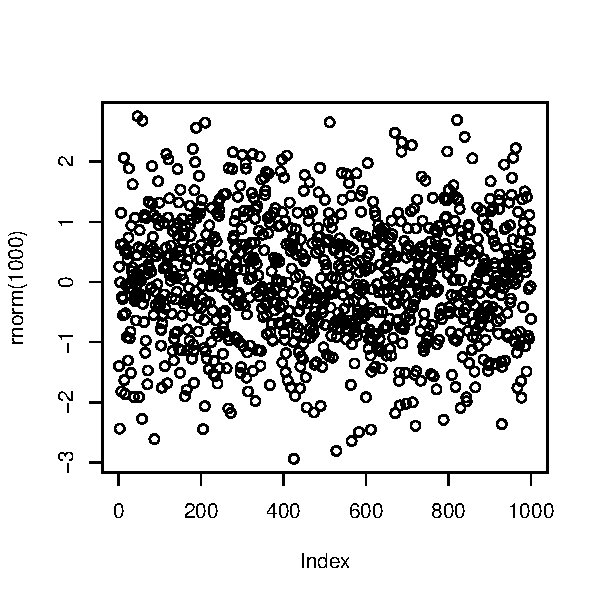
\includegraphics{figures/simple_plot-1.pdf}

Figure 1.1: Plot of 100 values randomly sampled from a normal
distribution.

Some of the best recent books on R include Hadley Wickham's `Advanced R'
(2014). He also has a very useful book on R packages (Wickham, 2015).

\section*{References}
\addcontentsline{toc}{section}{References}

Wickham, H. (2014). \emph{Advanced R}. CRC Press.

Wickham, H. (2015). \emph{R packages}. O'Reilly Media, Inc.
